% !TEX encoding = UTF-8 Unicode
\documentclass[a4paper]{article}

\usepackage{color}
\usepackage{url}
\usepackage[utf8]{inputenc}
\usepackage{graphicx}
\usepackage{amssymb}
\usepackage{amsmath}
\usepackage[english,serbian]{babel}

\usepackage[unicode]{hyperref}
\hypersetup{colorlinks,citecolor=green,filecolor=green,linkcolor=blue,urlcolor=blue}

\graphicspath{{../img/}}

\usepackage{minted}
\usemintedstyle{colorful}
\usepackage{listings}
\lstset{language=python}


\begin{document}

\title{Opasna zona oko vulkana\\ \small{Seminarski rad u okviru kursa\\ Osnove matematičkog modeliranja\\ Matematički fakultet, Beograd}}
\author{David Dimić, Sara Arsić\\ daviddimi@hotmail.com, saraarsic39@gmail.com}

\date{~Maj 2019.}

\maketitle

\abstract{
U ovom radu biće opisan postupak modeliranja jednog problema varijante kosog hica
ispaljenog sa zadate visine - određivanje sigurne zone oko vulkana koji izbacuje
užareno kamenje.
Postupna objašnjenja jednačina do kojih se došlo 
biće ilustrovana odgovarajućim slikama i jednom animacijom
isprogramiranih u programskom jeziku Python.
}

\tableofcontents

\newpage

\section{Uvod}
\label{sec:uvod}
Prvo će biti iznet problem koji se rešava, a potom pretpostavke u delu
\ref{sec:pretpostavke} koje su uzete da bi se problem lakše rešio. Kako je 
suštinski deo problema model kosog hica, on će biti pomenut u delu \ref{sec:kosi_hitac}
gde će biti izračunate neke ključne tačke za rešenje, a potom u poglavlju
\ref{sec:opasna_oblast} biće izneto rešenje problema. Na kraju će, u dodatku
\ref{sec:Dodatak}, biti prikazani kodovi korišćeni u ovom radu.

\subsection{Formulacija problema}
Vulkan na visini $h$ u odnosu na okolinu izbacuje užareno kamenje brzinom od maksimalno
$v_0$. Potrebno je odrediti zonu oko vulkana gde nije bezbedno leteti, kao i 
nebezbednu zonu u podnožju vulkana.


\subsection{Pretpostavke}
\label{sec:pretpostavke}
Radi lakšeg izračunavanja uzećemo u obzir sledeće pretpostavke. 
Za kosi hitac pretpostavljamo \cite{Drazic} da je kamen materijalna tačka 
sa nekom pozitivnom masom za koji u svakom trenutku možemo da izračunamo $x(t)$ i $y(t)$,
i da su ove funkcije dva puta neprekidno diferencijabilne, kako bismo mogli da primenimo
diferencijabilni i integralni račun. \\

Koordinatni sistem postavljemo u podnožje vulkana, u ravni zemlje, ispod njegovog otvora,
gde je $x$-osa u ravni zemlje, a $y$-osa u smeru vrha vulkana.
Otvor vulkana nalazi se na visini $h$ i iz te tačke može biti izbačen kamen pod bilo
kojim uglom $\alpha \in [0, \pi]$. Prvo ćemo posmatrati slučaj u ravni ovako postavljenog 
sistema, a potom uvesti i treću koordinatu, pošto kamen može biti ispaljen u bilo kom smeru. Još jedna važna pretpostavka je da užarena kugla u trenutku pada ostaje ukopana
na tom mestu (nema daljeg kotrljanja). U prostoru oko vulkana nema prepreki, a podnožje
smatramo ravnim. \\

Kako je maksimalna brzina pod kojom može da se izbaci kamen $v_0$, dozvoljene su sve brzine
između 0 i $v_0$. Pri modelovanju tražiće se maksimalna opasna zona, a 
sve trajektorije sa brzinom manje od maksimalne upašće u takvu zonu. Zbog ovoga će se svuda
nadalje koristiti da je brzina tačno $v_0$.

\section{Kosi hitac}
\label{sec:kosi_hitac}
Ispaljeni projektil sa visine $h$ početnom brzinom $v_0$ i pod uglom $\alpha$ u 
odnosu na $x$-osu možemo modelovati kosim hicem. Njegove parametarske jednačine su 
(za detaljno izvođenje pogledati \cite{Drazic}):

\begin{equation}
\label{eq:kosi_hitac_x}
x(t) = v_0 t \cos \alpha
\end{equation}
\begin{equation}
\label{eq:kosi_hitac_y}
y(t) = v_0 t \sin \alpha - \frac{gt^2}{2} + h
\end{equation}

Dalje ćemo odrediti koje su koordinate tačke gde se dostiže najveća visina, a potom,
gde se dostiže najdalji domet koji kosi hitac može da ima.


\subsection{Maksimalna visina}
\label{sec:max_visina}
Potražimo sada iz jednačina kosog hica \ref{eq:kosi_hitac_x} i \ref{eq:kosi_hitac_y}
gde izbačeni kamen pod uglom $\alpha$ dostiže maksimalnu visinu. Kako nas zanima 
maksimum funkcije po $y$-osi treba da važi:
$$ \frac{dy(t)}{dt} = 0 $$ 
$$ v_0 \sin \alpha - gt = 0 $$
odakle dobijamo vremenski trenutak $t_{max}$ u kojem se dostiže maksimum:
$$ t_{max} = \frac{v_0 \sin \alpha}{g} $$
zamenog ovog $t_{max}$ u jednačine kosog hica \ref{eq:kosi_hitac_x} i \ref{eq:kosi_hitac_y}
dobijemo koordinate traženog maksimuma. Označimo tu tačku sa $H$:
\begin{equation}
\label{eq:Hx}
H_{x} = \frac{v_0^2 \sin(2 \alpha)}{2g}
\end{equation}
\begin{equation}
\label{eq:Hy}
H_{y} = \frac{v_0^2 \sin^2 \alpha}{2g} + h
\end{equation}

Da bismo počeli sa određivanjem opasne zone, makar po $y$ kooridnati, 
potreno je rešiti za koji ugao $\alpha$ se dostiže maksimum? 
Kako nam je u jednačini \ref{eq:Hy} jedina promenljiiva ugao, 
to je očigledno kada sinus ima najveću vrenost,
a to je za $\alpha_{max} = \frac{\pi}{2}$ uzevši u obzir ograničenje 
da $\alpha \in [0, \pi]$. Onda je, uvrštavanjem ovog ugla u \ref{eq:Hy}
 najviša moguća tačka do koje kamen može da dobaci u visinu $H^{max}$:
\begin{equation}
\label{eq:Hmax_x}
H^{max}_{x} = 0
\end{equation}
\begin{equation}
\label{eq:Hmax_y}
H^{max}_{y} = h + \frac{v_0^2 }{2g}
\end{equation}
Radi jednostavnijeg zapisa u daljem tekstu $H_{max}$ označavaće $H^{max}_y$.

\begin{figure}[h!]
\begin{center}
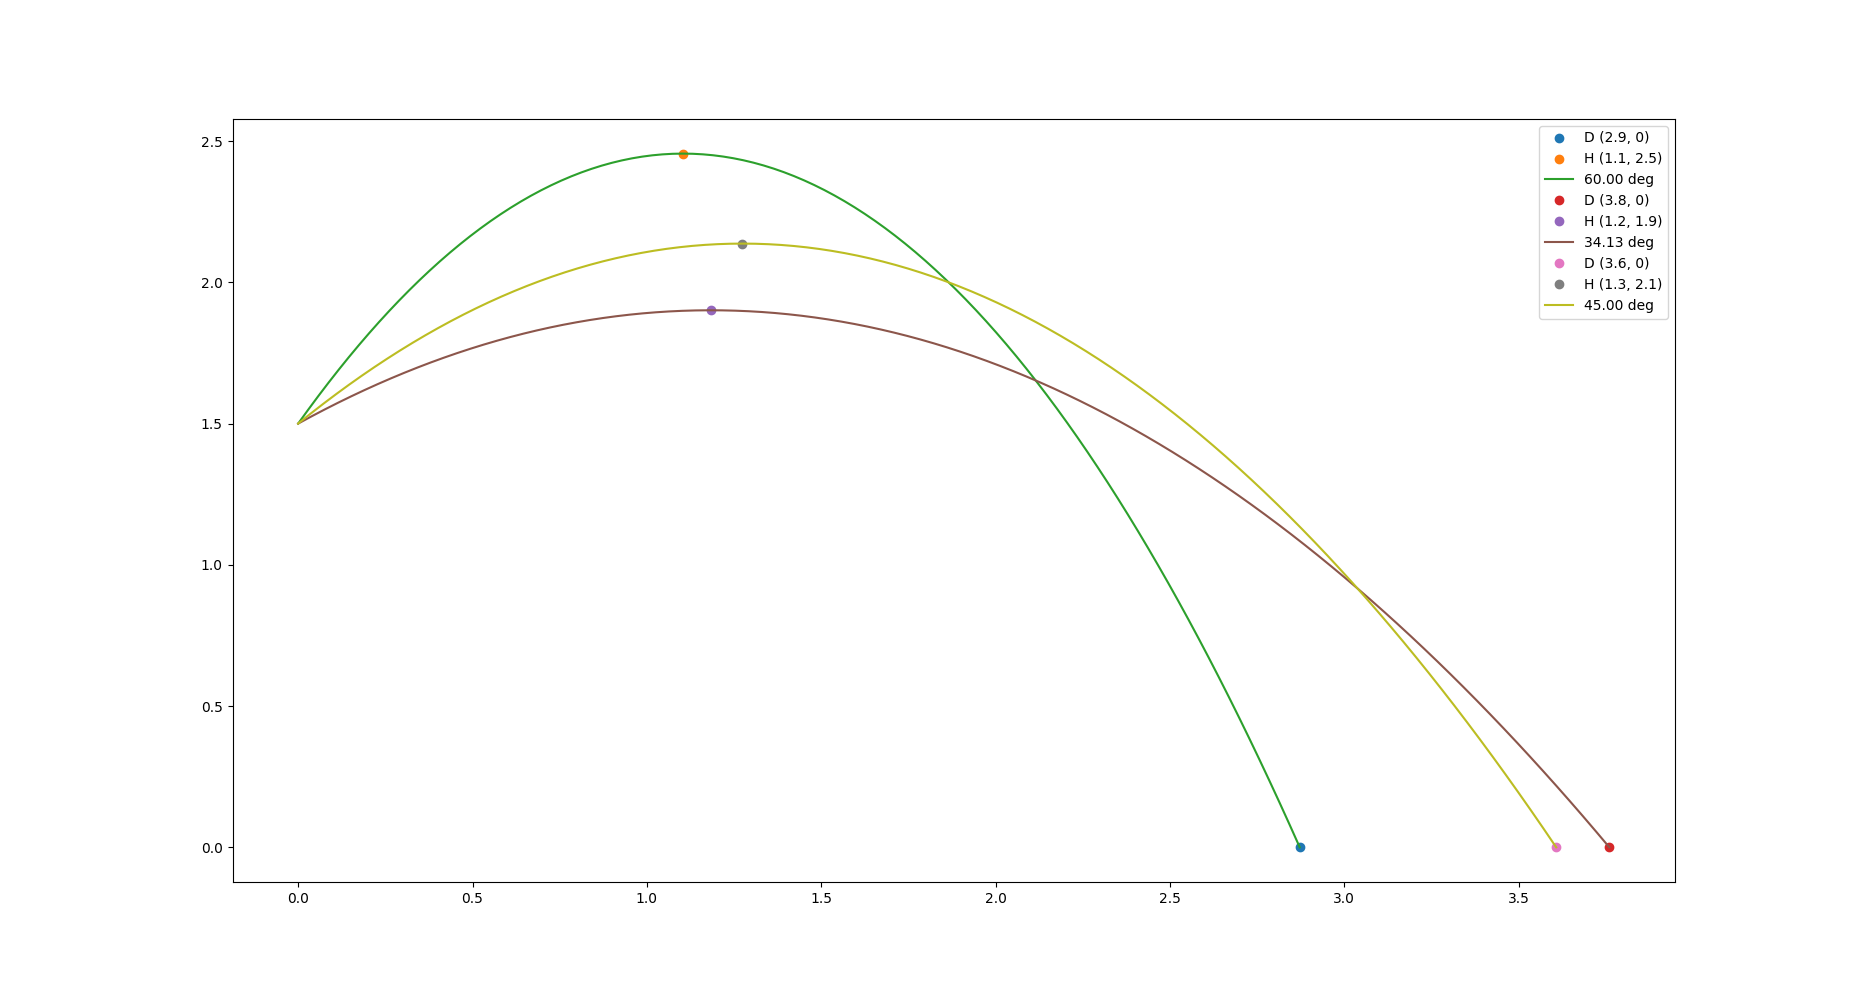
\includegraphics[width=\textwidth]{2D_hitac_vise.png}
\end{center}
\caption{Tri kosa hica sa označenima tačkama H i D}
\label{fig:kosi_hitac_tacke}
\end{figure}

\subsection{Maksimalni domet}
\label{sec:max_domet}
Odredimo koji je domet kamena izbačenog pod uglom $\alpha$, početnom brzinom $v_0$ sa 
vulkana visine $h$, odnosno trenutak kada pada na zemlju. 
Eliminacijom $t$ iz jednačine \ref{eq:kosi_hitac_x} i njenim uvrštavanjem 
\ref{eq:kosi_hitac_y} dobijamo jednačinu oblika $y=f(x)$, 
pri tome ikoristimo da je $1/\cos^2\alpha = 1+\tan^2\alpha$ 
i označimo $L = v_0^2/g$:
\begin{equation}
\label{eq:kosi_hitac_xy}
y = - x^2\frac{1+\tan^2 \alpha}{2L} + x \tan \alpha + h
\end{equation}
Označimo tačku dometa sa $D = x$.
Iz uslova da kamen treba da padne na zemlju važi da je $y = 0$, pa se dobija:
\begin{equation}
\label{eq:pocetak_sa_D}
D \tan \alpha - D^2\frac{1+\tan^2 \alpha}{2L} + h = 0
\end{equation}
Rešavanjem ove jednačine po $D$ dobile bi se dve tačke preseka sa $x$-osom: jedno pozitivno
i jedno negativno rešenje.
Negativno rešenje $D_1$ može da se razume kao tačka u prošlosti sa koje se, 
u nivou zemlje, bacio kamen čija trajektorija odgovara jednačini kosog hica. Drugo,
pozitivno rešenje predstavlja traženi domet $D$ kada ispaljeni kamen udara o zemlju.\\

Potražimo sada za koji ugao je taj domet maksimalan.
Posle izvoda po $\alpha$ na obe strane dobija se:
$$ \frac{dD}{d\alpha}\tan\alpha 
+ D \sec^2 \alpha - 
\left( \frac1L D \frac{dD}{d\alpha}(1+\tan^2\alpha) + 
\frac{1}{2L} D^2(2\tan\alpha \sec^2\alpha) \right) = 0 $$

$$ \frac{dD}{d\alpha} = 
\frac{D \sec^2\alpha(\frac{D}{L} \tan \alpha - 1)}
{\tan\alpha-\frac{D}{L}(1 + \tan^2 \alpha)} $$
Iz ove jednačine $D$ dostiže svoj maksimum za neki ugao $\alpha$ 
kada je $\frac{dD}{d\alpha} = 0$, odnosno kada je izraz
sa desne strane 0. Maksimum dometa se dostiže za:
$$ D_{max} \sec^2 \alpha (\frac{D_{max}}{L} \tan \alpha - 1) = 0 $$
$$ \frac{D_{max}}{L}\tan\alpha-1 = 0 $$
$$ \tan \alpha = \frac{L}{D_{max}} $$
Sada dobijeni $\tan \alpha$ zamenimo u formulu \ref{eq:pocetak_sa_D} i dobijamo:
$$ L - \frac{D_{max}^2}{2L} - \frac{L}{2} + h = 0 $$
$$ D_{max} = \sqrt{L^2 + 2Lh} $$
Dakle, tačka najdaljeg dometa je:
\begin{equation}
\label{eq:Dmax_x}
D^{max}_x = \sqrt{\left(\frac{v_0^2}{g}\right)^2 + 2h\frac{v_0^2}{g}}
\end{equation}
\begin{equation}
\label{eq:Dmax_y}
D^{max}_y = 0
\end{equation}
a ugao za koji se postiže najdalji domet $\alpha^{max}_{D}$:
\begin{equation}
\label{eq:Dmax_alpha}
 \alpha^{max}_{D} = \arctan \frac{1}{\sqrt{1 + \frac{2hg}{v_0^2}}}
\end{equation}


Na slici \ref{fig:kosi_hitac_tacke} označene su tačke $H$ i $D$ kosog hica, dok se
na slici \ref{fig:parabola} vide tačke $H^{max}$ i $D^{max}$ najdaljeg dometa po
kooridnatnim osama.


\section{Opasna oblast}
\label{sec:opasna_oblast}
U delu \ref{sec:max_visina} i \ref{sec:max_domet} izveli smo koje su najdalje tačke dometa
po $y$ ($H^{max}$ jednačine \ref{eq:Hmax_x} i \ref{eq:Hmax_y}), 
odnosno po $x$-osi ($D^{max}$ \ref{eq:Dmax_x} i \ref{eq:Dmax_y}). 
Potpuno simetrično u odnosu na $y$-osu, kamen može biti ispaljen ka negativnom delu
$x$-ose, pa je tada njegov maksimalni domet $-D^{max}$.\\

\begin{figure}[h!]
\begin{center}
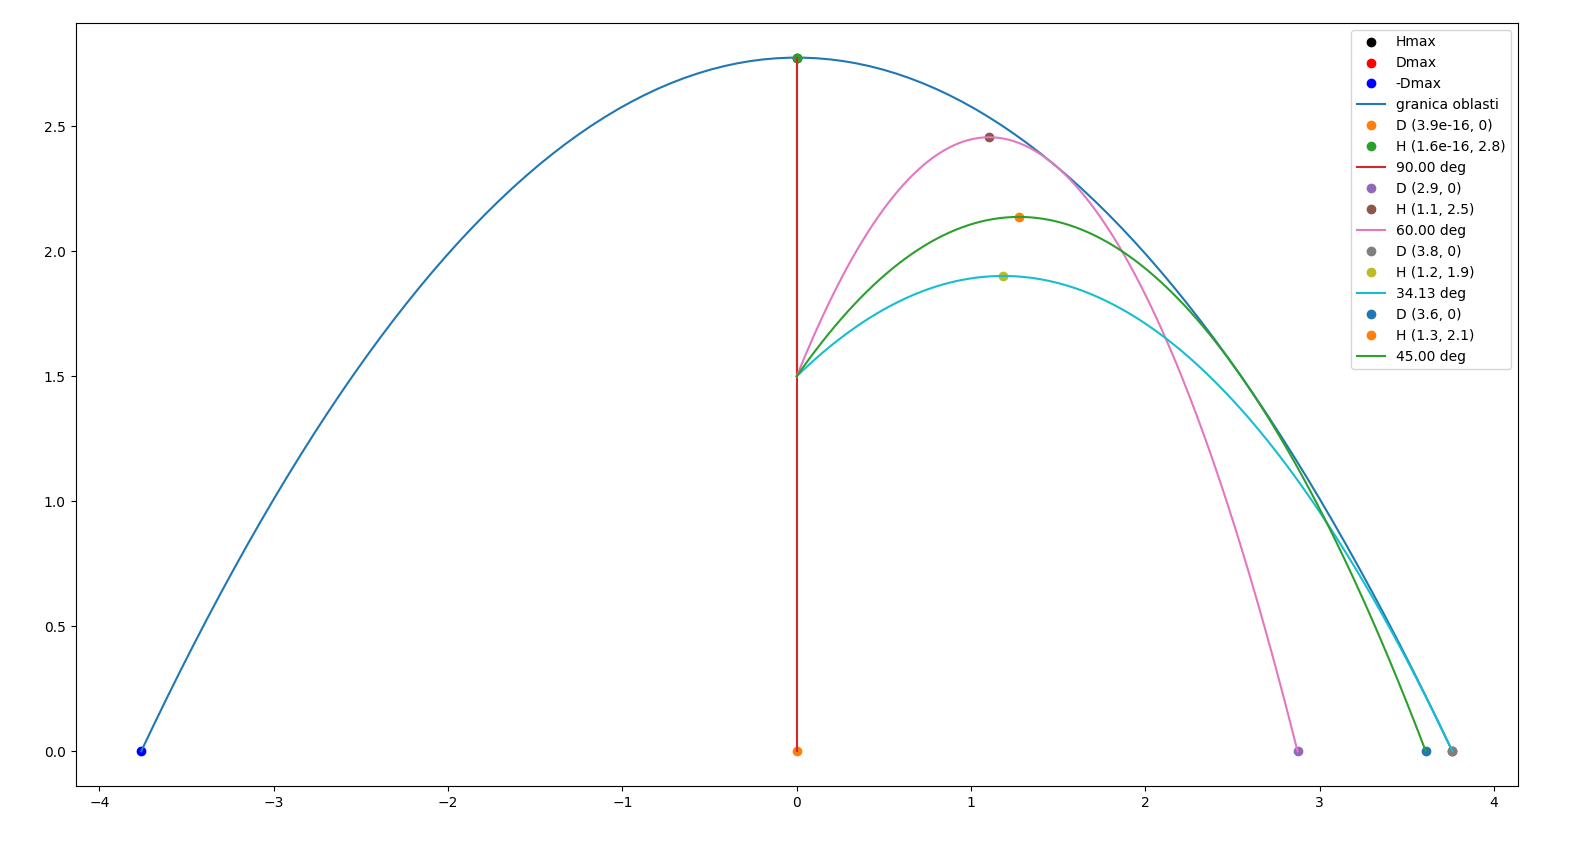
\includegraphics[width=\textwidth]{2D_parabola_vise.png}
\end{center}
\caption{Parabola opasne zone sa nekoliko trajektorija kamenja}
\label{fig:parabola}
\end{figure}

Varirajući ugao $\alpha$ dobijamo različite parabole, kao što je prikazano na slici 
\ref{fig:parabola}. Da bismo odredili sigurnu zonu potrebno je odrediti 
obvojnicu\footnote{Linija L koja u svakoj tački dodiruje samo jednu 
liniju familije krivih K, pri čemu u različitim tačkama dodiruje različite krive, 
zove se \textit{obvojnica} linija K.}
oko ove familije parabola.
Poznato je iz diferencijalne geometrije da se obvojnica neke familije ravanskih krivih
dobija kao rešenje sledećeg sistema jednačina:
\begin{equation}
\label{eq:obvojnica1}
F(x,y,a) = 0
\end{equation}
\begin{equation}
\label{eq:obvojnica2}
\frac{\partial F(x,y,a)}{\partial a} = 0
\end{equation}

U našem slučaju $F(x,y,a)$ je kriva \ref{eq:kosi_hitac_xy}, a parametar $a$ ugao $\alpha$.
Odnosno imamo sistem:
\begin{equation}
\label{eq:sistem1}
y + x^2\frac{1+\tan^2 \alpha}{2L} - x \tan \alpha - h = 0
\end{equation}
\begin{equation}
\label{eq:sistem2}
\frac{\partial F(x,y,\alpha)}{\partial \alpha} = 0
\end{equation}
Rešavajući prvo \ref{eq:sistem2} dobija se:
$$ x^2\frac{\tan \alpha\frac{1}{\cos^2 \alpha}}{L} - \frac{x}{\cos^2 \alpha} = 0 $$
odakle je $x$ koordinata obvojnice:
\begin{equation}
\label{eq:obvojnica_x}
x = \frac{L}{\tan \alpha}
\end{equation}
Uvrštavajući ovo $x$ u prvu jednačinu sistema \ref{eq:sistem1} dobija se i $y$ kooridnata
obvojnice:
\begin{equation}
\label{eq:obvojnica_y}
y = h + \frac{L}{2} - \frac{L}{2 \tan \alpha}
\end{equation}

Da bismo dobili jednačinu obvojnice paraboli kosog hica sa parametrom $\alpha$, iz
\ref{eq:obvojnica_x} izrazićemo $\tan \alpha$ i uvrstiti u \ref{eq:obvojnica_y},
pri čemu je $h + L/2 = H_{max}$: 
\begin{equation}
\label{eq:obvojnica_kriva}
y = H_{max} - \frac{x^2}{2L}
\end{equation}

Ovim je pokazano da je obvojnica takođe jedna parabola. Na slici \ref{fig:parabola}
vidi se njen grafik i da ona zaista jeste granična kriva opasne oblasti vulkana.
K\^od ove slike opisan je u delu \ref{kod:2D_oblast}.\\


Kako kamen može biti ispaljen u ma kojem pravcu, rotacijom dobijene parabole oko
$y$-ose dobija se paraboloid koji opisuje nebezbedan prostor oko vulkana.
Uvrštavanjem tačke maksimuma i prečnika oblasti u podnožju u jednačinu paraboloida
$ 2p(z-z_0) = (x-x_0)^2 + (y-y_0)^2 $ dobija se tražena površ:
\begin{equation}
\label{eq:paraboloid1}
z = H_{max} - \frac{1}{2L} (x^2 + y^2)
\end{equation}
a kako je $1/(2L) = H_{max}/D^2_{max}$, možemo ovu oblast zapisati preko
maksimalnih tačaka dometa po koordinatnim osama koje smo izračunali u 
\ref{sec:max_domet} i \ref{sec:max_visina}:
\begin{equation}
\label{eq:paraboloid}
\boxed{z = H_{max} - \frac{H_{max}}{D^2_{max}} (x^2 + y^2)}
\end{equation}

\begin{figure}[h!]
\begin{center}
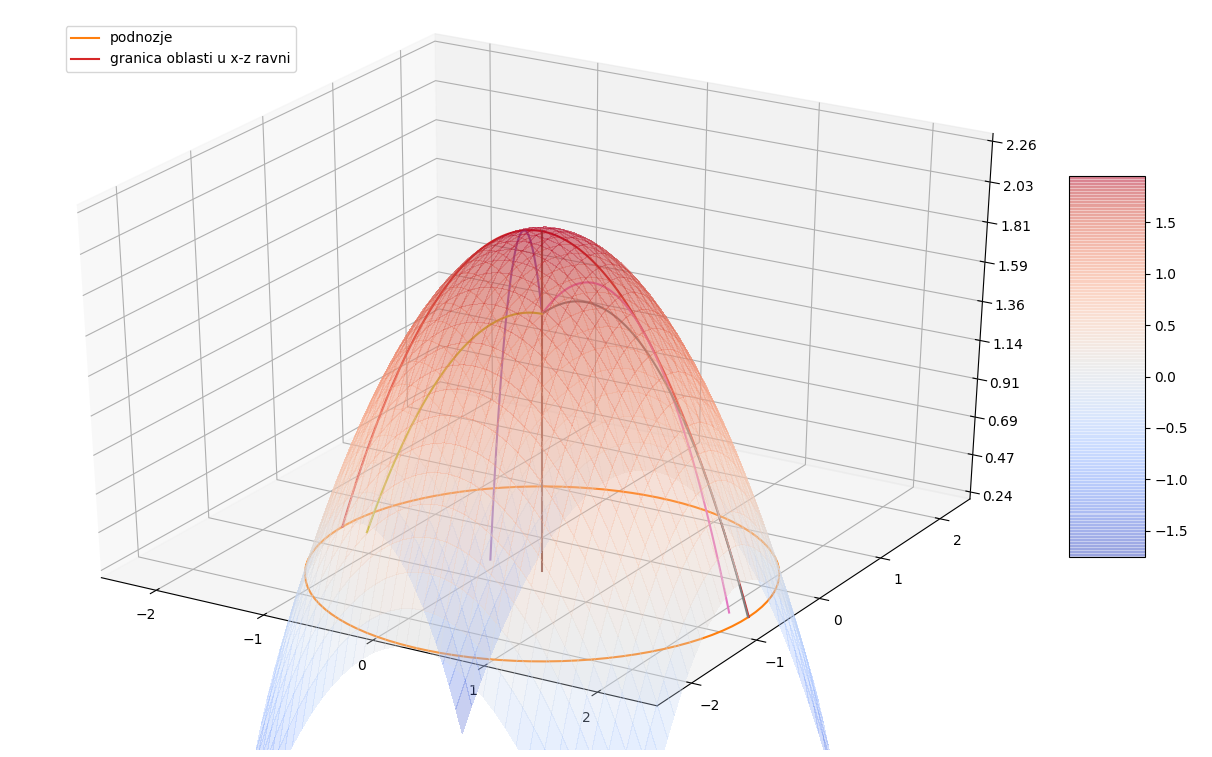
\includegraphics[width=\textwidth]{opasna_oblast.png}
\end{center}
\caption{Opasna zona sa nekoliko trajektorija kamenja}
\label{fig:paraboloid}
\end{figure}

Na slici \ref{fig:paraboloid} prikazana je ova površ kao i zona u podnožju.
Za nekoliko uglova ($\pi, \frac{\pi}{1.8}, \frac{\pi}{2}, \frac{\pi}{4}, 
\frac{\pi}{6} $) iscrtane su trajektorije kamenja koje u jednoj tački dodiruju
površ, ali je nikada ne presecaju. K\^{o}d za generisanje slike dat je u dodatku
\ref{kod:oblast}.\\

Kada je $z=0$ u jednačini \ref{eq:paraboloid} dobija se očekivana opasna zona 
u podnožju vulkana - krug poluprečnika
$D_{max}$:
\begin{equation}
x^2 + y^2 = D^2_{max}
\end{equation}


\section{Zaključak}
\label{sec:zakljucak}
U ovom radu predstavljen je jedan način za određivanje opasne zone oko vulkana koji
izbacuje užareno kamenje. Data je formulacija problema i nekoliko pretpostavki koje su 
napravljene radi lakšeg modeliranja, iskorišćen je ključni koncept kosog hica
za modelovanje trajektorije kamenja. Izvedene su formule ekstremnih tačaka 
po $x$ i $y$ osi i iskorišćene za određivanje, prvo granice oblasti u
$\mathbb{R}^2$, što je jedna parabola, a potom njeno proširenje na paraboloid u 
$\mathbb{R}^3$ čime se dobilo finalno rešenje problema. 
Celokupan rad i sve formule propraćene su proverom u programskom jeziku
\verb|Python| kojim su generisane slike i jedna animacija, čiji su kodovi
dati u dodatku.


\addcontentsline{toc}{section}{Literatura}
\appendix
\bibliography{seminarski} 
\bibliographystyle{plain}

\appendix
\section{Dodatak - k\^{o}dovi}
\label{sec:Dodatak}
Pri izradi rada i proveri dobijenih jednačina korišćen je programski jezik 
\verb|Python| i modul \verb|matplotlib|
za sve slike i animacije koje se nalaze u radu. 
Ovde će biti izloženi korišćeni kodovi uz kratka objašnjenja. 
Svi kodovi takođe su dostupni na GitHub nalogu autora 
\footnote{\url{https://github.com/daviddimic/opasna-zona-oko-vulkana}}.

\subsection{Kosi hitac i granična parabola u ravni}
\label{kod:2D_oblast}
Naredni k\^od generiše nekoliko parametrizovanih paraboli kosog hica, pri čemu
su svi parametri osim ugla $\alpha$ fiksirani. Označene su ključne tačke
izračunate u delu \ref{sec:max_domet} i \ref{sec:max_visina}. Prikazana je i
parabola koja određuje granicu opasne zone oko vulkana.
\begin{minted}{python}
import matplotlib.pyplot as plt
import numpy as np

fig, ax = plt.subplots()
# Parametri kosog hica
g = 9.81
v0 = 5
h = 1.5
# Kljucne tacke maksimuma
Hmax = h + v0**2/(2*g)
Dmax_sq = (v0**2/g)**2 + 2*h*v0**2/g
Dmax = np.sqrt(Dmax_sq)

def plot_tacke():
    ax.plot(0, Hmax, 'o', color='black', label = 'Hmax')
    ax.plot(Dmax, 0, 'o', color='red', label = 'Dmax')
    ax.plot(-Dmax, 0, 'o', color='blue', label = '-Dmax')

def plot_hitac(alpha):
    """
    Iscrtavanje parabole kosog hica sa uglom alpha
    i tackama kada dostize max visina i max domet
    """
    # Dt je vreme kada telo pada na zemlju
    Dt = (v0*np.sin(alpha) + np.sqrt((v0**2)*(np.sin(alpha))**2 + 2*g*h))/g
    t = np.linspace(0, Dt, 100)
    x = v0*t*np.cos(alpha)
    y = v0*t*np.sin(alpha) - g*t**2/2 + h
    # Tacke max visine i max dometa
    D = v0*np.cos(alpha)*Dt
    ax.plot(D, 0, 'o', label = 'D (%0.2g, %0.2g)' % (D, 0))
    Hx = v0**2*np.sin(2*alpha)/(2*g)
    Hy = h + v0**2*np.sin(alpha)**2/(2*g)
    ax.plot(Hx, Hy, 'o', label = 'H (%0.2g, %0.2g)' % (Hx, Hy))
    ax.plot(x, y, label = '%0.2f deg' % (alpha*180/np.pi))

def plot_parabola():
    """
    Crtanje parabole opasne oblasti
    """
    x = np.linspace(-Dmax,Dmax,100)
    y = -(Hmax/Dmax_sq)*x**2 + Hmax
    ax.plot(x, y, label = 'granica oblasti')

plot_tacke()
plot_parabola()
plot_hitac(np.pi/2)
plot_hitac(np.pi/3)
# Za ovaj ugao je maksimalni domet
plot_hitac(np.arctan(1/np.sqrt(1+2*h*g/v0**2)))
plot_hitac(np.pi/4)
ax.legend(loc='upper right')
plt.show()
\end{minted}

\subsection{Opasna oblast u prostoru}
\label{kod:oblast}
Sledeći program generiše sliku na kojoj je prikazana opasna oblast oko vulkana,
nekoliko trajektorija kosog hica za različite uglove, kao i granica te oblasti u 
podnožju. Vidi se da svaka od putanja kamenja dodiruje granicu oblasti u jednoj tački.

\begin{minted}{python}
from mpl_toolkits.mplot3d import Axes3D
import matplotlib.pyplot as plt
from matplotlib import cm
from matplotlib.ticker import LinearLocator, FormatStrFormatter
import numpy as np

fig = plt.figure()
ax = fig.gca(projection='3d')
line, = ax.plot([], [], lw=2)
# Podesavanja koordinatnih osa
ax.set_xlim(-3, 3)
ax.set_ylim(-3, 3)
ax.set_zlim(0, 2.5)
# z-osa
ax.zaxis.set_major_locator(LinearLocator(10))
ax.zaxis.set_major_formatter(FormatStrFormatter('%.02f'))

# Parametri kosog hica
g = 9.81
v0 = 3
h = 1.5
# Kljucne tacke maksimuma
Hmax = h + v0**2/(2*g)
Dmax_sq = (v0**2/g)**2 + 2*h*v0**2/g
Dmax = np.sqrt(Dmax_sq)

y = np.zeros(100)

def plot_podnozje():
    t = np.linspace(0, 2*np.pi, 100)
    x = Dmax*np.cos(t)
    z = Dmax*np.sin(t) 
    ax.plot(x, z, y, label = 'podnozje')

def plot_hitac(alpha):
    """
    Iscrtavanje parabole kosog hica u x-z ravni sa uglom alpha
    """
    #Dt - vreme kada telo pada na zemlju
    Dt = (v0*np.sin(alpha) + np.sqrt((v0**2)*(np.sin(alpha))**2 + 2*g*h))/g
    t = np.linspace(0, Dt, 100)
    x = v0*t*np.cos(alpha)
    z = v0*t*np.sin(alpha) - g*t**2/2 + h
    ax.plot(x, y, z)

def plot_parabola():
    """
    Crtanje parabole opasne oblasti u x-z ravni
    """
    x = np.linspace(-Dmax,Dmax,100)
    z = -(Hmax/Dmax_sq)*x**2 + Hmax
    ax.plot(x, y, z, label = 'granica oblasti u x-z ravni')

def plot_paraboloid():
    """
    Iscrtavanje paraboloida opasne oblasti
    """
    X = np.arange(-Dmax, Dmax, 0.1)
    Y = np.arange(-Dmax, Dmax, 0.1)
    X, Y = np.meshgrid(X, Y)
    Z = Hmax - (X**2 + Y**2)/(Dmax_sq/Hmax)
    surf = ax.plot_surface(X, Y, Z, cmap=cm.coolwarm, 
                          linewidth=0, antialiased=False, alpha=0.3)
    # color bar
    fig.colorbar(surf, shrink = 0.5, aspect = 5)

plot_podnozje()
plot_paraboloid()
plot_parabola()
plot_hitac(np.pi/1.8)
plot_hitac(np.pi/2)
plot_hitac(np.pi/4)
plot_hitac(np.pi/6)
plot_hitac(np.pi)
ax.legend(loc='upper left')
plt.show()
\end{minted}


\subsection{Animacija}
\label{kod:animacija}
Sledeći primer k\^{o}da prikazuje da je dobijena nebezbedna oblast zaista tačno rešenje
datog problema 
\footnote{\url{https://raw.githubusercontent.com/daviddimic/opasna-zona-oko-vulkana/master/img/vulkan_animation.mp4}}. 
Svi parametri kosog hica su fiksirani osim ugla $\alpha \in [0,\pi]$ 
koji je parametar animacije. Kosi hitac se iscrtava u $x$-$z$ ravni radi dobre 
vidiljivosti, ali zbog simetrije, on može biti usmeren u bilo kom pravcu oko $z$-ose.
Zbog dodatne jasnoće u istoj ravni sa kosim hicem iscrtana je i parabola koja
predstavlja granicu dobijene oblasti. Cilj animacije je prikazati da parabola kosog hica,
kada se provarila ugao $\alpha$, tačno opisuje parabolu granice 
tražene oblasti oko vulkana. Funkcije {\mintinline{python}{plot_parabola()}},
{\mintinline{python}{plot_paraboloid()}} i {\mintinline{python}{plot_podnozje()}}
su iste kao u prethodnom primeru \ref{kod:oblast}, 
pa je ovde njihova definicija izostavljena.

\begin{minted}{python}
from mpl_toolkits.mplot3d import Axes3D
from matplotlib import cm
import numpy as np
from matplotlib import pyplot as plt
from matplotlib import animation

fig = plt.figure(figsize=(12, 10))
ax = fig.add_subplot(111, projection='3d')
line, = ax.plot([], [], lw=2)
# Podesavanja koordinatnih osa
ax.set_xlim(-2, 2)
ax.set_ylim(-2, 2)
ax.set_zlim(0, 2)
# Parametri kosog hica
g = 9.81
v0 = 3
h = 1.5
# Kljucne tacke maksimuma
Hmax = h + v0**2/(2*g)
Dmax_sq = (v0**2/g)**2 + 2*h*v0**2/g
Dmax = np.sqrt(Dmax_sq)

y = np.zeros(100)

def init():
    """
    Inicijalizacija animacije
    """
    line.set_data([], [])
    line.set_3d_properties([])
    return line,

def animate(i):
    """
    Funkcija koja se poziva pri svakom frejmu animacije
    """
    alpha = i/100
    #Dt - vreme kada telo pada na zemlju
    Dt = (v0*np.sin(alpha) + np.sqrt((v0**2)*(np.sin(alpha))**2 + 2*g*h))/g
    t = np.linspace(0, Dt, 100)
    x = v0*t*np.cos(alpha)
    z = v0*t*np.sin(alpha) - g*t*t/2 + h
    
    line.set_data(x, y)
    line.set_3d_properties(z)
    line.set_color('red')
    return line,

# Animacija
anim = animation.FuncAnimation(fig, animate, init_func = init,
                               frames = 300, interval = 20, blit = True)
plot_podnozje()
plot_parabola()
plot_paraboloid()
ax.legend(loc='upper left')
plt.show()
\end{minted}


\end{document}
